%%%%%%%%%%%%%%%%%%%%%%%%%%%%%%%%%%%%%%%%%%%%%%%%%%%%%%%%%%%%%%%%%%%%%%%%%%%%%%%
% **IMPORTANT** remarks ahead
% - linelength <= 80 (in the text, unless unavoidable)
% - no TABs
% - no trailing spaces
% - Use macros for more complicated variables
%   (especially, if the notation might be changed later...)
%%%%%%%%%%%%%%%%%%%%%%%%%%%%%%%%%%%%%%%%%%%%%%%%%%%%%%%%%%%%%%%%%%%%%%%%%%%%%%%

\documentclass[reprint,superscriptaddress,amsmath,amssymb,aps,pre]{revtex4-1}

\usepackage{graphicx}% Include figure files
\graphicspath{plots}
\usepackage{dcolumn}% Align table columns on decimal point
\usepackage{bm}% bold math
\usepackage{color}
\usepackage{bbold}
\usepackage{soul}

\usepackage{empheq}
\setcounter{topnumber}{1}

\usepackage{flafter}     % Bilder immer nach \figure Befehl


% http://tex.stackexchange.com/questions/62010/can-i-access-system-environment-variables-from-latex-for-instance-home
\usepackage{catchfile}
\newcommand{\getenv}[2][]{%
\CatchFileEdef{\temp}{"|kpsewhich --var-value #2"}{\endlinechar=-1}%
\if\relax\detokenize{#1}\relax\temp\else\let#1\temp\fi}

%\getenv[\HOME]{HOME}


% use okular to view this file and acroread will be called on links
%\newcommand{\articlestoragepath}{/home/scratch/abaecker/ArticleStorage/}
\getenv[\articlestoragepath]{ARTICLE_STORAGE}
% Conditionally import pdf_article_link.sty to ensure that it works
% even without this file.
\IfFileExists{pdf_article_link.sty}{\usepackage{pdf_article_link}}

\input defs.tex
\newcommand{\overbar}[1]{\mkern 1.5mu\overline{\mkern-1.5mu#1\mkern-1.5mu}\mkern 1.5mu}

%%%%%%%%%%%%%%%%%%%%%%%%%%%%%%%%%%%%%%%%%%%%%%%%%%%%%%%%%%%%%%%%%%%%%%%%%%%%
% ADD THE FOLLOWING COUPLE LINES INTO YOUR PREAMBLE
\let\OLDthebibliography\thebibliography
\renewcommand\thebibliography[1]{
  \OLDthebibliography{#1}
  \setlength{\parskip}{0pt}
  \setlength{\itemsep}{0pt plus 0.3ex}
}



\makeatletter
\let\Hy@backout\@gobble
\makeatother


%%%%%%%%%%%%%%%%%%%%%%%%%%%%%%%%%%%%%%%%%%%%%%%%%%%%%%%%%%%%%%%%%%%%%%%%%%%%%%%
\begin{document}



\title{Mechanism to control synchronization in coupled area-preserving maps}

\author{Swetamber Das}
\affiliation{Max-Planck-Institut f\"ur Physik komplexer Systeme, N\"othnitzer
    Stra\ss{}e 38, 01187 Dresden, Germany}

\date{\today}

\begin{abstract}
 A unidirectionally coupled area-preserving maps with mixed phase space may 
show identical synchronization in the sticky neighborhood of the regular 
islands. We use this fact to devise a couple of numerical procedures to 
delay and expedite the process of synchronization in standard maps coupled 
under  Pecora-Caroll coupling scheme. The delay method is based on controlled 
kicking of trajectories away from synchronization traps for as long as 
necessary. On the other hand, the method to expiate the process is
achieved by a parameter perturbation technique which rapidly drives the 
chaotic trajectories to synchronization traps in the sticky neighborhoods 
of regular islands. We also point out of the limitations of these methods.
\end{abstract}

\pacs{PACS here}

\maketitle

\section{Introduction} 
Low-dimensional Hamiltonian systems commonly exhibit mixed phase space i.e. 
regular structures and chaotic regions may co-exist at a given degree of 
nonlinearity. This mixed nature has interesting consequences for the transport
properties of such systems, for instance, the existence of anomalous kinetics,
L\'{e}vy processes and L\'{e}vy flights \cite{Klafter1994,Zaburdaev2015}, 
power law contributions to recurrence and other statistics, and the existence 
of dynamical traps \cite{Zaslavsky2002a,Zaslavsky2002b}. An interesting region 
of a mixed phase space is the interface between regular regions and chaotic 
sea \cite{Mackay1984, Easton1993}. The dynamics in these neighbourhoods are 
complex but fairly well understood \cite{Meiss2015} for lower dimensional 
systems. The complexity arises from the fact that a chaotic trajectory spends 
an arbitrary long but finite time at the boundaries of regular islands before 
exiting to the chaotic sea. The intermittent tendency of chaotic trajectories 
to stay close to the regular boundaries is called the phenomenon of 
stickiness. A major consequence of the stickiness is  the existence of power 
law in the Poincar{\'e} recurrence times indicating algebraic decay for long 
times times rather than exponential decay expected for normal transport. 
Therefore, due to stickiness, even a small regular island can influence the 
global transport properties of the system and decay of correlations. The 
phenomenon has been of great interest and continues to be studied on 
theoretical level \cite{Altmann2006, Altmann2010,Livorati2012,Bunimovich2012, 
Kruger2015}. In addition, stickiness has found application in several problems 
such as particle advection in fluids \cite{Babiano1994,Tel2005}, transport in 
plasma fusion devices \cite{Szezech2012,Martins2014}, celestial mechanics 
\cite{Efthymiopoulos1999, Harsoula2010, Harsoula2016}.

A recent feature of stickiness has emerged from a connected quarter. In our 
recent work~\cite{Mahata2016}, we have looked at the effects of the mixed 
phase space on the synchronization in a system of two standard maps coupled in 
unidirectional drive-response configuration. We have shown that 
synchronization of chaotic trajectories of the drive and response maps 
typically occurs in the neighborhood of regular inlands as a consequence of 
stickiness in the region.  This is the first instance, as far as we are aware, 
where stickiness have been found to influence synchronization in coupled 
chaotic systems.  For a chaotic orbit, synchronization typically happens via 
an intermittent behavior in the phase difference of the drive and response 
maps.   The sticky neighborhoods of a regular islands contain dynamical traps 
in chaotic orbits. In such trapping regions in the phase space, parts of a 
chaotic trajectory are almost regular in time and allow for synchronization to 
occur. Such traps are characterized using the properties of the finite-time 
Lyapunov exponent \cite{Szezech2005}. In the context of our work, we will 
refer to these traps as synchronization traps. We further noted that the 
behavior of the synchronization traps can be analyzed in a more quantitative 
way by analyzing the location and stability properties of the periodic orbits 
in the vicinity of the locations where synchronization takes place.

Synchronization in coupled chaotic systems, coupled map lattices and networks 
have been studied in great details over the years. Coupled Hamiltonian systems are also known to show synchronization such as measure synchronization~\cite{Hampton1999,Wang2003,Vincent2005,Gupta2017} and identical synchronization~\cite{Mahata2016,Das2017} The fact however remains 
that the ability to control synchronization based on the dynamics of the 
process has not been given much attention, until 
recently~\cite{Grabow2011,Wang2016}. In realistic systems, the speed of 
synchronization may be significant. For example, in
neurosciences,  the speed of the visual and olfactory processing are 
interesting problems \cite{Thorpe1996,Uchida2003}. In this paper, we intend 
to develop a couple of 
mechanisms to control synchronization process to wit,  to increase and to 
decrease synchronization times based on the location of synchronization traps 
in the sticky neighborhood of regular islands in the phase space of the 
area-preserving system of the standard map. We demonstrate the mechanism at $K 
= 6$ where only two small regular islands exist. It is important to point out 
that the role of stickiness in Hamiltonian systems for synchronization was 
already predicted by Zaslavsky~\cite{Zaslavsky2002b} early in the last decade.

The rest of the paper is 
organized in the following way: we explain the coupling scheme in 
sec.~\ref{sec:Pecora_Carroll} and the mechanism based on the location of 
synchronization traps is given in sec.~\ref{Master stability function}. The 
numerical procedures to delay and advanced synchronization times are 
demonstrated in sec.~\ref{sec:delay} and sec.~\ref{sec:advanced} respectively, 
and the paper ends with conclusions in sec.~\ref{sec:conclusions} including 
discussion on limitations and implications. 


\section{The Pecora Caroll's unidirectional coupling scheme}
\label{sec:Pecora_Carroll} 
The standard map is considered to be the prototypical example of a two-dimensional area-preserving map, and is given by:

\begin{empheq}[right=\empheqrbrace \mod 1]{align}
P_{n+1} = P_n +  \frac{K}{2\pi}\sin(2\pi Q_n) \nonumber\\
Q_{n+1} = P_{n+1} + Q_n 
\end{empheq}

\begin{figure}[b]
	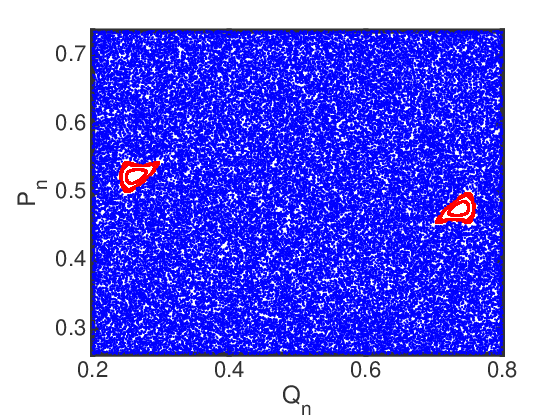
\includegraphics[scale=.45]{Standard_Map}
	\caption{\label{fig:Standard_map} \footnotesize The phase space of the standard map for  random initial conditions from the uniform distribution on $[0,1]$,  at the parameter value K = 6.0.}
\end{figure}
Here the subscript $n$ denotes the discrete time and $K$ is the nonlinearity parameter. These equations typically describe the evolution of two canonical variables $P$ and $Q$ which correspond to the momentum and co-ordinate in the Poincar\'{e} section of a freely moving rotator with interleaved periodic kicks. This system represents the behavior of a variety of systems such as charged particle confinement in  mirror magnetic traps, particle dynamics in accelerator, comet dynamics in solar systems etc.  Two-dimensional  phase space plots  of the standard map for the parameter value $K = 6$ using $25$ initial conditions  are shown in Figs.~\ref{fig:Standard_map}.


We now synchronize two standard maps, using the Pecora-Carroll scheme of synchronization using drive-response coupling \cite{Pecora1990,Pecora2015}. 
This system was first devised to synchronize the chaotic trajectories dissipative chaotic dynamical systems. Under this unidirectional coupling scheme, we duplicate the given map and couple the original and the duplicated map in a drive-response configuration. This means that the drive map evolves freely but the evolution of the response map is dependent on the drive. In this case, the $P$ value of the response system is set to the $P$ value of the drive system, at each iterate.  Therefore, the coupled system is described by the following equations

\begin{minipage}[t]{0.5\textwidth}
	\begin{empheq}[right=\empheqrbrace \mod 1]{align}\nonumber
	\label{equ:drive}
	P^d_{n+1} = P^d_n + \frac{K}{2\pi}\sin(2\pi Q^d_n)\nonumber\\
	Q^d_{n+1} = P^d_{n+1} + Q^d_n \nonumber
	\end{empheq}
	\centering \textbf{(Drive)}
	
\end{minipage}
\begin{minipage}[t]{0.5\textwidth}
	\begin{empheq}[right=\empheqrbrace \mod 1]{align}
	P^r_{n+1} = P^d_n + \frac{K}{2\pi}\sin(2\pi Q^r_n) \nonumber \\
	Q^r_{n+1} = P^r_{n+1} + Q^r_n \nonumber
	\end{empheq}
	\centering \textbf{(Response)}
\end{minipage}

\vspace{.5cm}

The initial values of $Q$ in the drive and response maps are chosen arbitrarily, whereas the $P$ values are identical. The system is said to reach complete synchronization when both the $Q$ values of the drive and response systems evolve asymptotically to identical values i.e. 
\begin{equation}
\lim_{t\rightarrow\infty}(Q^d_n - Q^r_n) = 0
\end{equation}

Synchronization time is the least value of the iterate say, $\tau$, where $\Delta Q = Q^d-Q^r$ vanishes and remains so for rest of the iterations. 
\begin{equation}
(Q^d_n - Q^r_n) = 0; \hfill  n \geq  \bf {\tau }
\end{equation}

In all of the computations reported in the work, two chaotic trajectories are considered to be synchronized to numerical accuracy, if the Euclidean distance between them is less than $10^{-5}$. An example is shown in Fig.~\ref{fig:sync_ex}. Here, we plot $\Delta Q = Q^d_n-Q^r_n$ for initial conditions $(P^d_0,Q^d_0,Q^r_0) = (0.569, 0.906,0.106)$ at $K = 6$. The synchronization time is found to be 570246. 

\begin{figure}[t]
	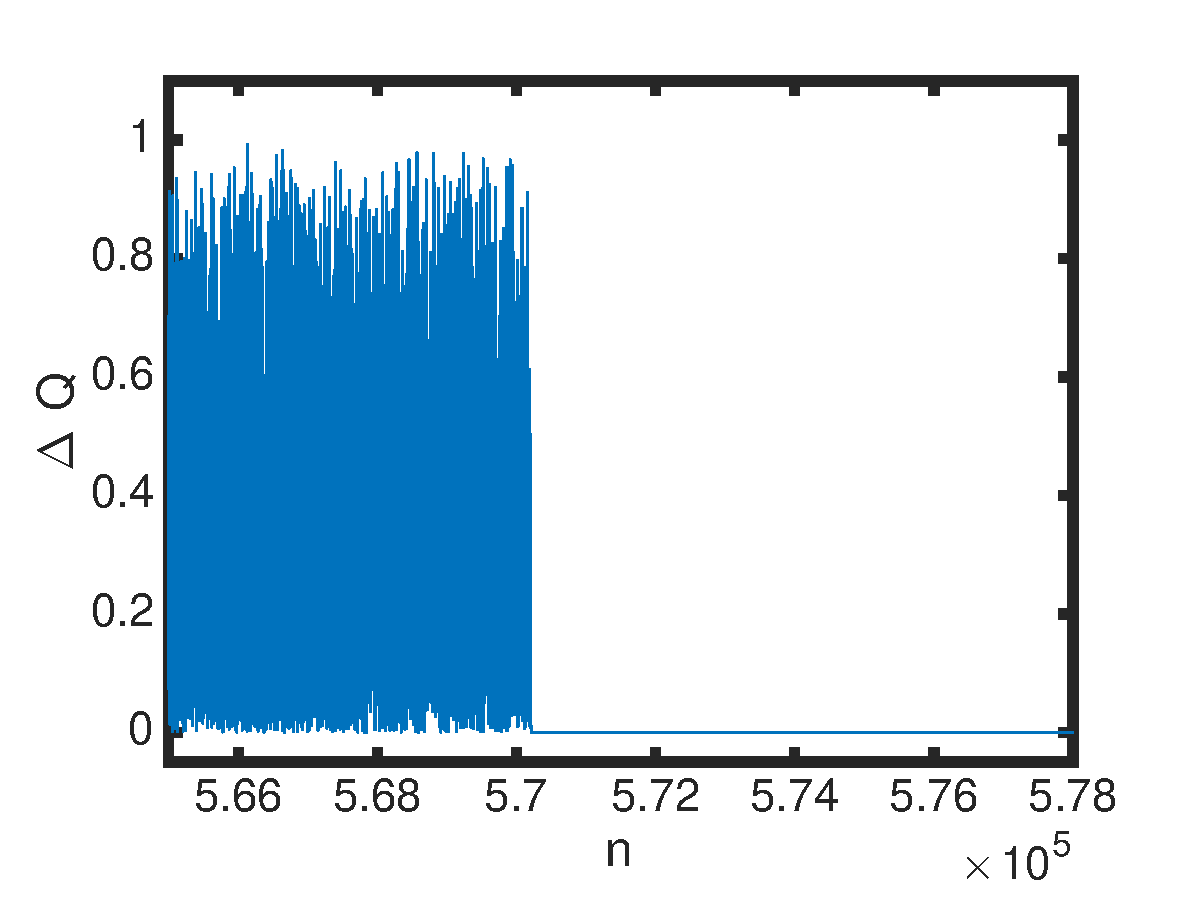
\includegraphics[scale=.4]{Sync_exmaple}
	\caption{\label{fig:sync_ex} \footnotesize The variation of $\Delta Q = Q^d_n-Q^r_n$ of the coupled system at $K = 6$ with iterations $n$. Synchronization is considered to be achieved when $\Delta Q < 10^{-5}$ and remain so for the rest of the iterations. The iteration step $n$ at which synchronization occurs is called synchronization time $\tau$. For this case, $\tau = 570 246.$ }
\end{figure}

We now analyze synchronization of the coupled system using the master stability function~\cite{Pecora1998}. The numerical procedures to control synchronization times will be discussed thereafter.  

\section{Locating Synchronization Traps using Master stability function}
\label{Master stability function}
A general drive-response system coupled unidirectionally may be described by the following set of equations

\begin{align}
\frac{d\overbar{X}_d}{dt} = \overbar{F}(\overbar{X}_d) \nonumber  &&
\frac{d\overbar{X_r}}{dt} = \overbar{F}(\overbar{X}_r) + \alpha E(\overbar{X}_d-\overbar{X}_r)
\end{align}

Here $\overbar{X}_d$ and $\overbar{X}_r$ are drive and response variables; the matrix $E$ determines the linear combination of the $\overbar{X}$ used in the difference and $\alpha$ is the coupling strength. For the map case, we have the following form

\begin{align}
\overbar{X}^d_{n+1} = \overbar{F}(\overbar{X}^d_{n}) \nonumber  &&
\overbar{X}^r_{n+1} = \overbar{F}(\overbar{X}^r_{n}) + \alpha E(\overbar{X}^d_{n}-\overbar{X}^r_n)
\end{align}

Therefore, in the case of a general unidirectional coupling of two standard maps, we get
\begin{align}
P^d_{n+1} &= P^d_n + \frac{K}{2\pi}\sin(2\pi Q^d_n) \nonumber\\
Q^d_{n+1} &= P^d_{n+1} + Q^d_n \nonumber\\
P^r_{n+1} &= P^r_n + \frac{K}{2\pi}\sin (2\pi Q^r_n) + \alpha(P^d_n-P^r_n) \nonumber \\
Q^r_{n+1} &= P^r_{n+1} + Q^r_n 
\label{equ:coupled}
\end{align}


We have chosen $E$ to be the matrix $\begin{bmatrix} 1 & 0 \\ 1 & 0 \end{bmatrix}$. 

To find the stability of the synchronous state, we first express  Eq.(\ref{equ:coupled}) in terms of  $P^\perp = P^d - P^r$ and $Q^\perp = Q^d - Q^r$, as follows
\begin{eqnarray}
\label{equ:trans}
P^\perp_{n+1} = (1-\alpha)P^\perp_n+ \frac{K}{2\pi} \sin(2\pi Q^d_n) - \frac{K}{2\pi} \sin(2\pi Q^r_n) \\ \nonumber
Q^\perp_{n+1} = (1-\alpha)P^\perp_n+ Q^\perp_n + \frac{K}{2\pi} \sin(2\pi Q^d_n) - \frac{K}{2\pi} \sin(2\pi Q^r_n)  
\end{eqnarray}

We now write the variational equation for Eq.(\ref{equ:trans}) by linearizing about $(P^d_n,Q^d_n)$
\begin{equation}
\label{equ:variational}
\left[ \begin{array}{c} \delta P^\perp_{n+1} \\ \delta Q^\perp_{n+1} \end{array} \right] = \mathcal{M}(\alpha)\left[ \begin{array}{c}\delta P^\perp_{n} \\ \delta Q^\perp_{n} \end{array} \right]
\end{equation}
where the matrix $\mathcal{M}(\alpha)$ is given by
\begin{equation} 
\label{equ:M}
\mathcal{M}(\alpha) = \begin{bmatrix} 1-\alpha & K\cos(2\pi Q^d_n) \\ 1 - \alpha & 1 + K\cos(2\pi Q^d_n) \end{bmatrix} 
\end{equation}

This is the master stability equation for the unidirectionally coupled standard map. The variational equation (\ref{equ:variational}) is the master stability equation for the coupled system under investigation. The associated largest LE computed from the master stability equation is the master stability function of the system, given by:
\begin{equation}
\label{equ:msf}
\lambda  = \lim_{n \rightarrow \infty} \lim_{\delta\overbar{X}_0\rightarrow 0}\frac{1}{n}\sum^{n-1}_{i=0}\ln|JM^n(\overbar{X}_i)|
\end{equation}

Here $n$ is a positive integer and $JM^n(\overbar{X}_i)$ denotes the Jacobian matrix of the $n$-times iterated map.  A negative value of the MSF (the largest non-zero LE) will ensure that $(P^\perp,Q^\perp) $ tend to zero indicating that the difference between $P$ and $Q$ will die out and the system will synchronize. 
Now, for the Pecora-Carroll approach, we set $\alpha = 1$. This substitution simplifies the matrix in Eq.(\ref{equ:M}) which now reads

\begin{equation} 
\mathcal{M}(1)= \begin{bmatrix} 0 & K\cos(2\pi Q^d_n) \\ 0 & 1 + K\cos(2\pi Q^d_n) \end{bmatrix} 
\end{equation}

The MSF should then be computed from the eigenvalues of the matrix $\mathcal{M}(1)$. It is easy to see that, for $\alpha =1$, one of the eigenvalues of   $\mathcal{M}(1)$ is zero. Therefore, we need to consider only the non-zero eigenvalue which is $1+K\cos(2\pi Q^d_n)$. The corresponding LE is given by

\begin{equation}
\label{equ:LE}
\lambda   = \lim_{n \rightarrow \infty} \frac{1}{n}\sum^{n-1}_{i=0}\ln|1+K\cos(2\pi Q^d_n)|
\end{equation}

In general, we define the $kth$ time-$n$ Lyapunov exponent associated with an initial point $\overbar{X}_0 = (P_0,Q_0)$ for a map $M(P,Q)$ as
\begin{equation}
\label{equ:FLEf}
\lambda _k(\overbar{X}_0;n)  = \frac{1}{n}\sum^{n-1}_{i=0}\ln|JM^n(\overbar{X}_i)|
\end{equation}

\begin{figure*}[t!]
	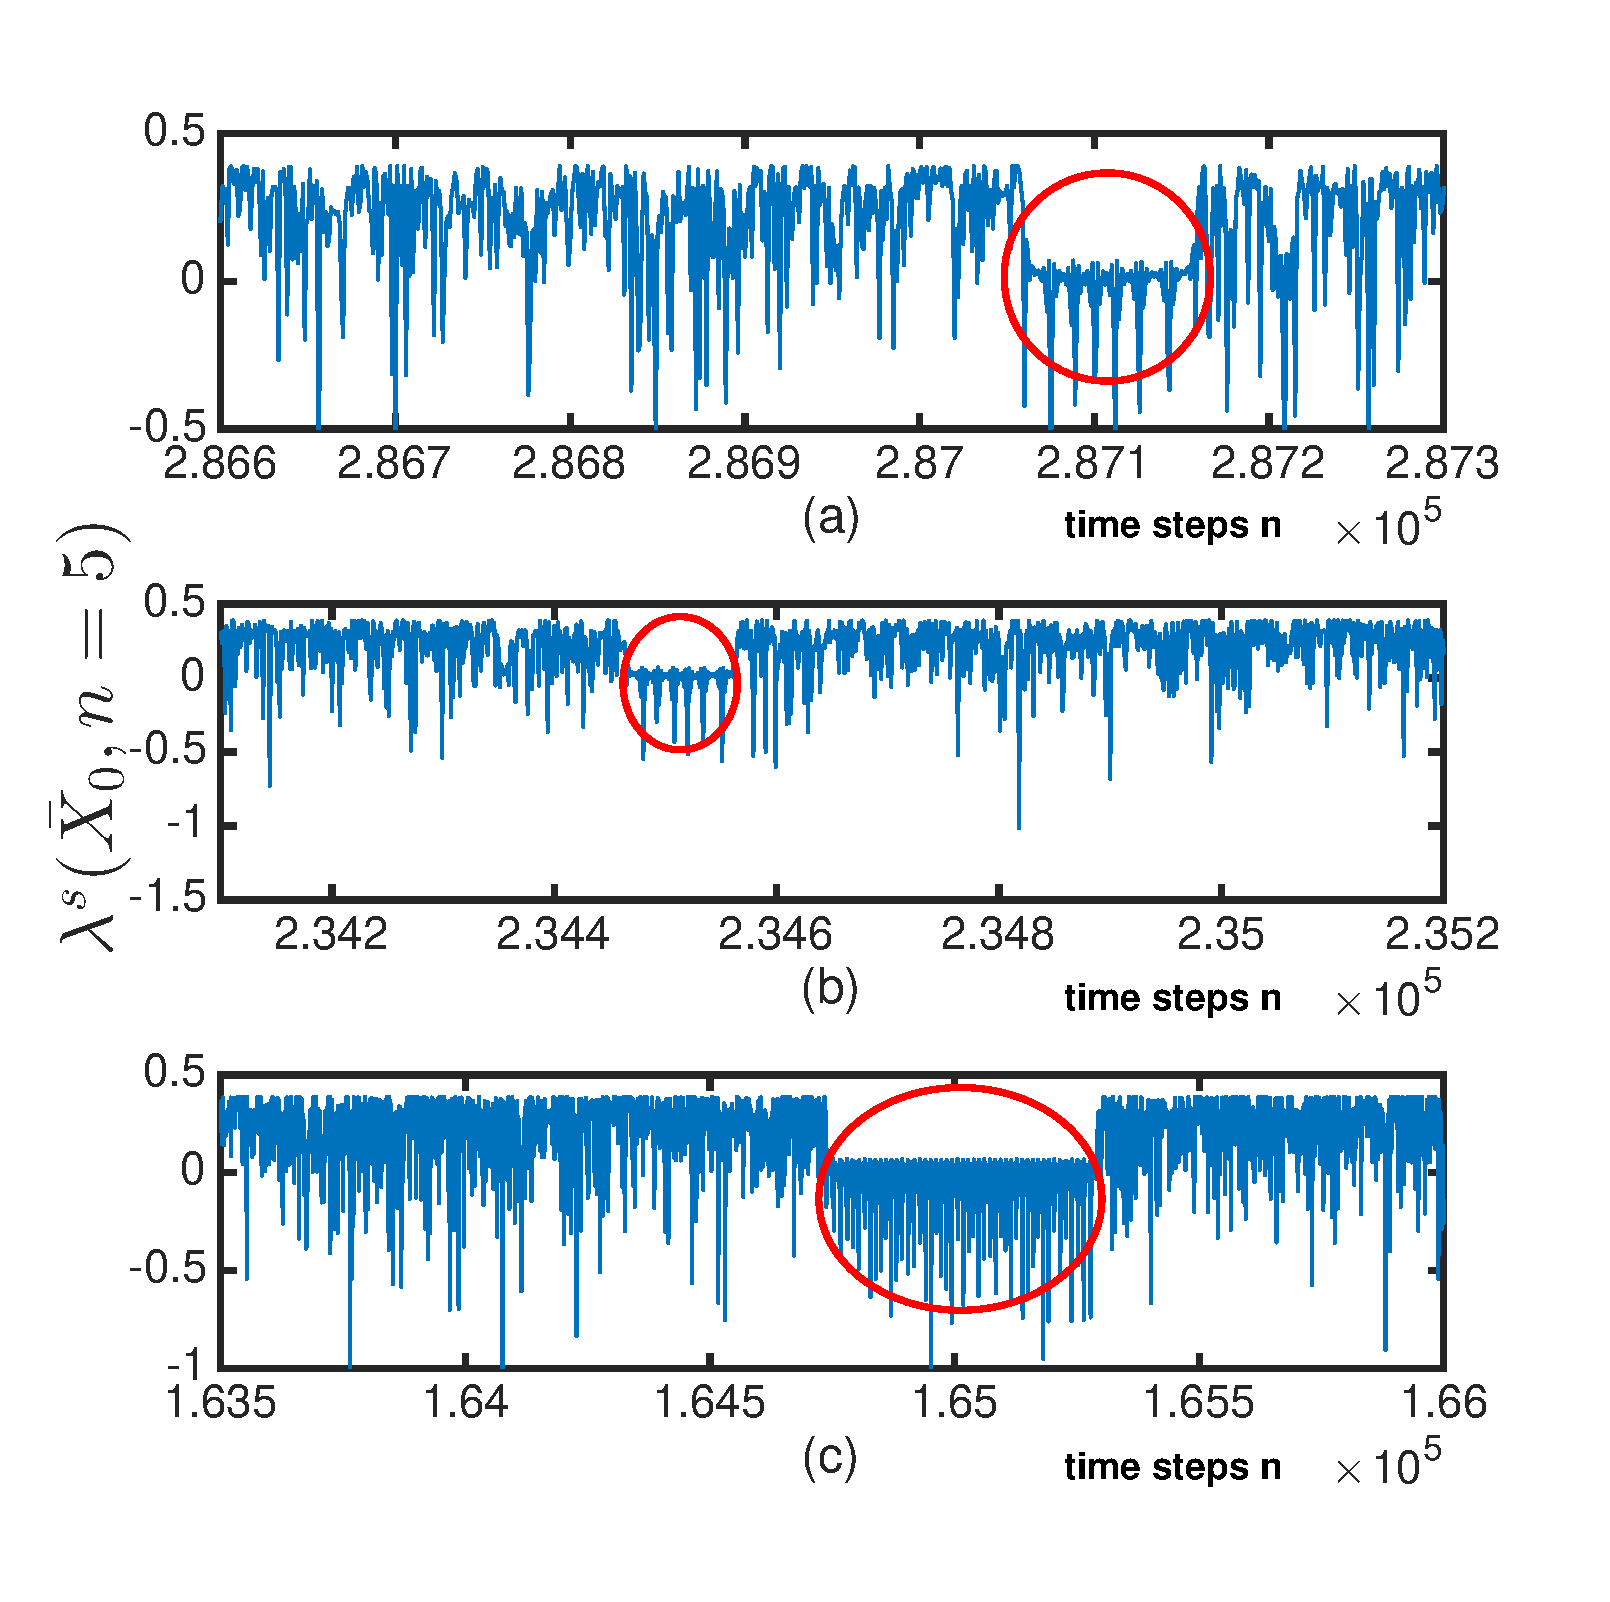
\includegraphics[scale=0.41]{FTLE_plots}
	\caption{\label{fig:FTLE}\footnotesize Fluctuations of time-5 FTLEs for three different set of initial conditions -- $(P^d_0,Q^d_0,Q^r_0) = (0.466,0.098,0.141)$ in (a),  $(0.009,0.026,0.129)$ in (b), and $(0.553,0.554,0.396)$ in (c). The synchronization times in each cases are 287090, 234521, and 164782 respectively. The time scale on the x-axis indicates iterates steps $t$ at which time-5 FTLEs have been computed. The drop window in (a), (b), and (c) shown in ellipses in red occur around synchronization times. Synchronization of chaotic trajectories in the coupled system under study typically occurs in one of such traps.}
\end{figure*}

Here $n$ is a positive integer and $JM^n(\overbar{X}_i)$ denotes the Jacobian matrix of the $n$-times iterated map. We extend this notion to the master stability function defined in the Sec.~\ref{Master stability function}  i.e.  the non-zero Lyapunov exponent defined in Eq.(\ref{equ:LE}) 
which takes the following finite time version 
\begin{equation}
\lambda_1^s(\overbar{X}_0;n) = \frac{1}{n}\sum^{n-1}_{i=0}\ln|1 + K \cos (2\pi Q_i)|
\end{equation}

The subscript ($k = 1$) has been dropped hereafter as we have only one LE to compute.

We plot the variation in the time-5 FTLE defined above at $K = 6$. At the point of synchronization, the FTLE values attain a set of negative values consistently in a small window, indicating the existence of a synchronization trap.  In Fig.~\ref{fig:FTLE} , the three plots show the fluctuations  of FTLE near the point of synchronization for three different sets of initial conditions - $(P^d_0,Q^d_0,Q^r_0) = (0.466,0.098,0.141)$ in (a),  $(0.009,0.026,0.129)$ in (b), and $(0.553,0.554,0.396)$ in (c) with synchronization times 287090, 234521, and 164782 respectively. The values on the x-axis indicate time steps at which averages are computed so that synchronization times and the temporal neighborhood are effectively captured in the plots wherein a temporary drop is clearly visible, indicated by ellipses in red. Synchronization of chaotic trajectories typically occurs in one of such traps. 

\section{Delayed Synchronization Times}
\label{sec:delay}
In order to develop a numerical technique to delay synchronization, we  first 
have to identify the vicinity of regular islands in the phase space. A 
mechanism  to suppress stickiness based on the knowledge of hyperbolic and non 
hyperbolic regions in the phase has been reported recently~\cite{Kruger2015}. 
Our method, however, targets the trajectories themselves in the sticky region 
to delay the process.  It is to be noted that the proposed procedure ignores 
the details of a rather complex hierarchy of structures around regular 
islands. We employ the edge-detection algorithm due to Benkadda {\it et al.} 
\cite{Benkadda1997} to identify the edges of regular islands in phase space. 
For the numerical procedure, we divide the phase space in $100 \times 100$ 
grid. The edges of both the islands are detected by applying the standard map 
to point initiated in the chaotic sea, for $10^7$ times.  The edges thus 
detected in shown in Fig~\ref{fig:edge_reg_island}.  We have chosen the 
thickness parameter to be $d=0.02$ i.e. euclidean distance of $d$ from points 
on the edge indicate the extent of the vicinity of the island.  This vicinity, 
therefore, indicate the domain wherein the synchronization traps exist.  To 
demonstrate this explicitly, we compare the phase angles, defined by $\theta = 
\tan^{-1}(\frac{Q}{P}$), of the points on the numerically detected edges and 
the points of synchronization, as 
follows.

\begin{figure}[b]
    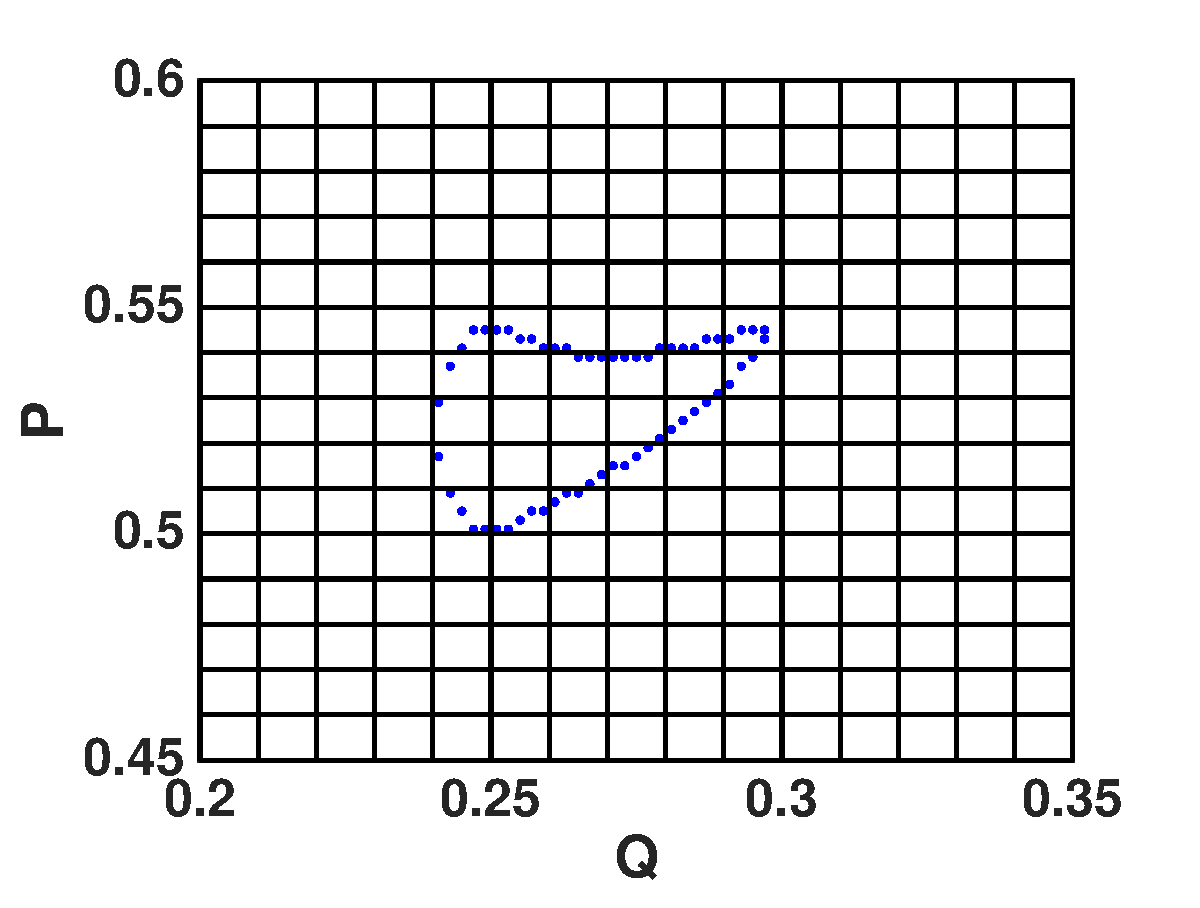
\includegraphics[scale=0.42]{edge_reg_island.eps}
    %\includegraphics[scale=.4]{Standard_Map2.eps}\\
    \caption{\label{fig:edge_reg_island} \footnotesize Example to detect the 
    edge of a regular island in the phase space using edge detection 
    algorithm  due to Benkadda {\it et al.} \cite{Benkadda1997}. }
\end{figure}

In Fig.~\ref{fig:Edge_Sync_angles}(a), we show the distribution of phase angles of the points on the edges of regular islands determined by the edge-detection algorithm.  The bimodality of the distribution is due to the existence of two sharp islands in otherwise chaotic bulk in the phase space.  We compare this with the phase angles corresponding to the points in the phase space at which synchronization of the chaotic trajectories occurs.


\begin{figure}[h]
	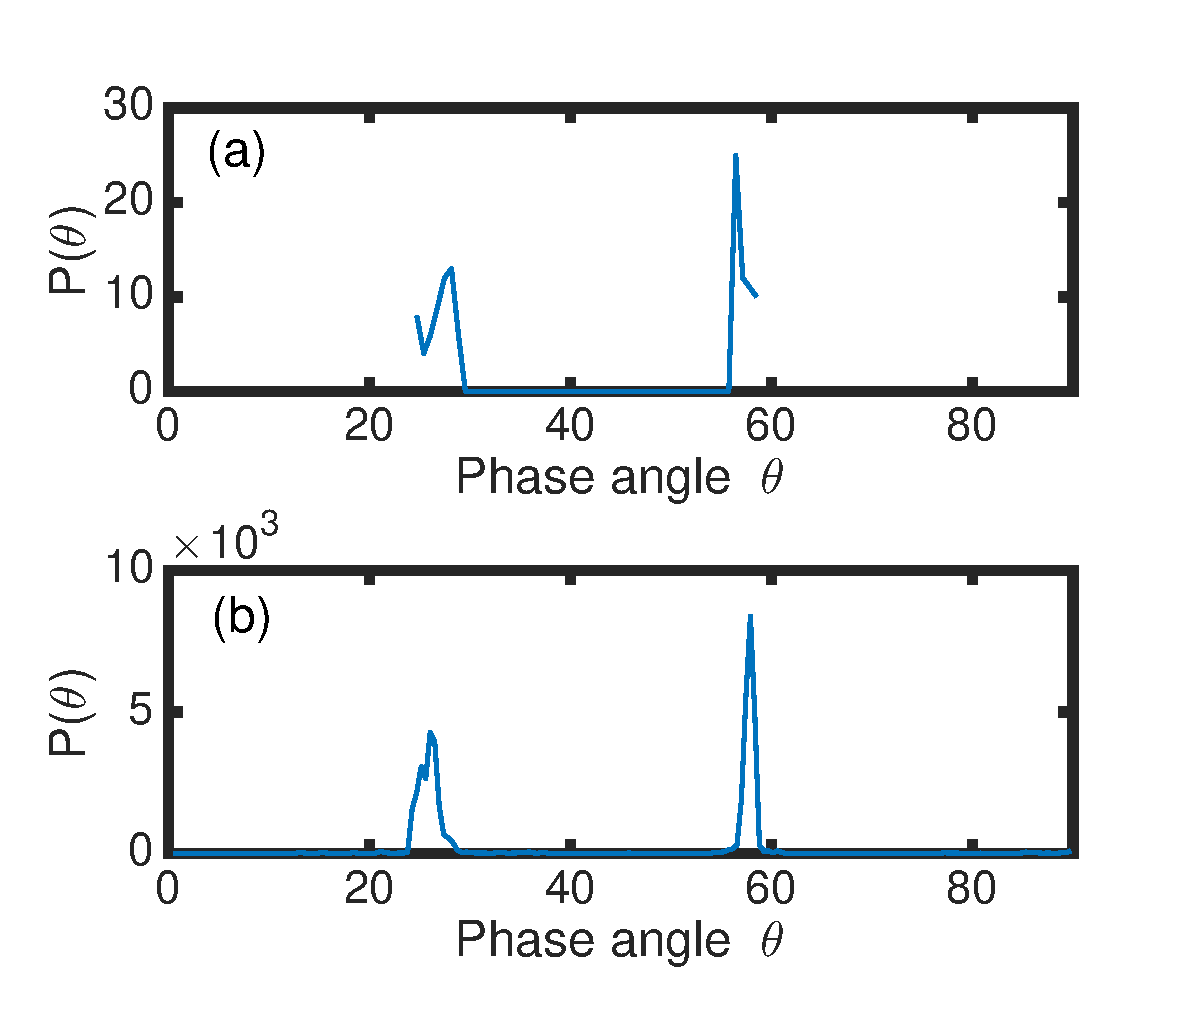
\includegraphics[scale=0.45]{Edge_Sync_angles}
	%\includegraphics[scale=.4]{Standard_Map2.eps}\\
	\caption{\label{fig:Edge_Sync_angles} \footnotesize Numerical detection of 
		synchronization traps (a) Distribution of phase 
		angles of the points on the edges of regular islands determined by the edge 
		detection algorithm. (b) Distribution of phase angles for points where 
		synchronization occurs. }
\end{figure}

Fig.~\ref{fig:Edge_Sync_angles}(b) shows the distribution of these phase angles for about 50 000 randomly chosen initial conditions for the drive and response maps that lead to synchronization. The locations of the peaks in the distribution shown in (a) approximately matches with this in (b). It is, therefore, visibly clear that synchronization occurs in the same angular domain of the phase space where the regular islands exist. Our numerically detected edges, thus correctly locate the synchronization traps in the phase space.  We now discuss the control mechanism to delay synchronization time. 

The proximity parameter $d_0 = 0.02$ defines the region in the neighborhood of 
the numerically detected edges wherein synchronization traps exist. The basic 
idea to control synchronization time is to identify the step at which the 
chaotic trajectory visits the numerically determined sticky neighborhood 
followed by a slight deflection so that the trajectory restarts at a point 
outside.  Our procedure depends upon how many times we deflect the trajectory  
which will be referred to as step control. This means that if an $n-$step 
control is  employed then, the trajectory will be kicked away from the domain 
$n$-times during its first $n$ visits i.e. once per visit. The deflection is 
achieved by adding a randomly generated fraction below $0.1$ to the point 
visiting the domain, and therefore the maximum deflection area is roughly 
$1\%$ of the phase space.  This procedure applied on a given set of initial 
conditions of the drive and response maps, may result in four possibilities of 
synchronization time -- (1) successful delay  \textbf{(S)}, (2) no delay 
\textbf{(N)}, (3) failed to achieve synchronization \textbf{(F)}, and (4) 
undesirable faster synchronization \textbf{(U)}. Clearly, the only first 
possibility is the aim of the mechanism; the last one constitute a hazard 
while the other two are trivial. 
\begin{figure}[h]
	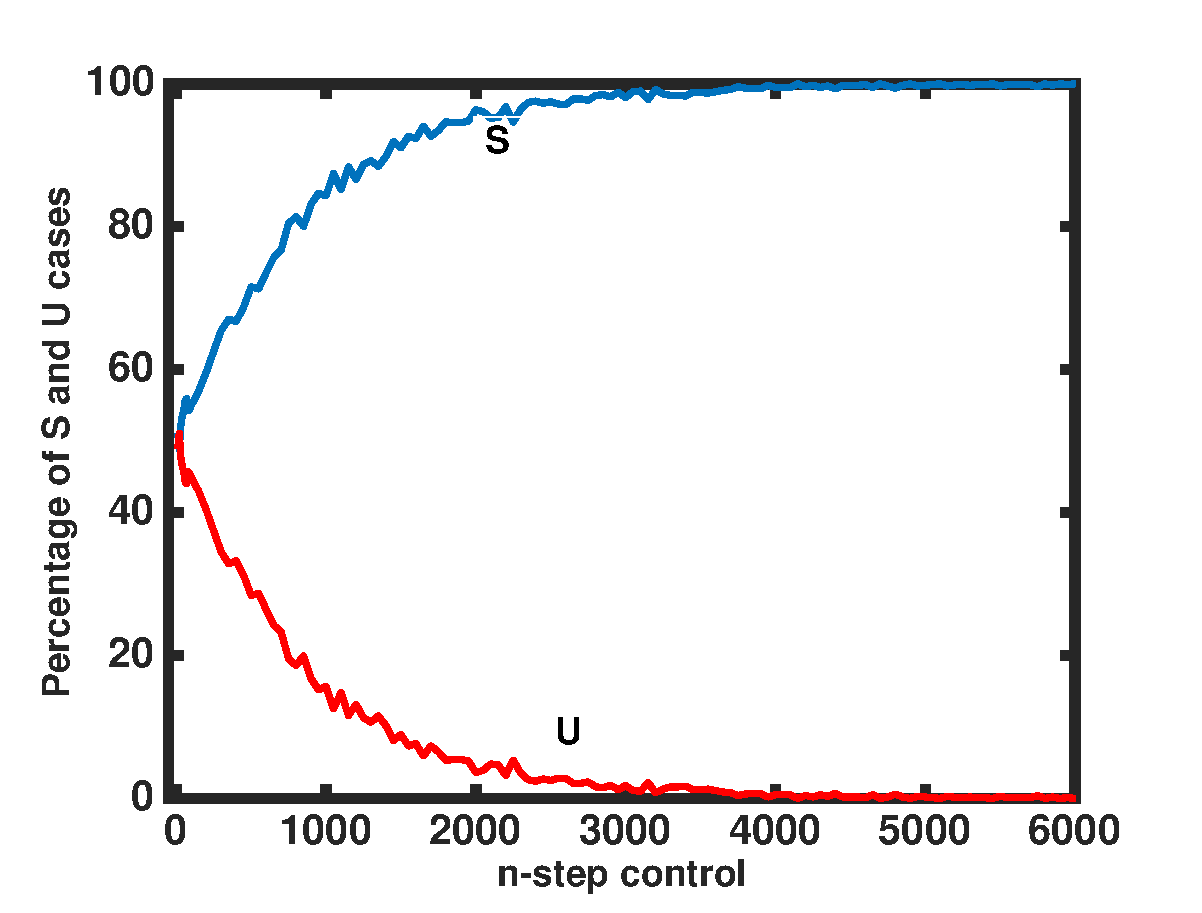
\includegraphics[scale=0.45]{S_U_Percent}
	\caption{\label{fig:Control_success}\footnotesize The curves indicate the 
		percentages of (S) successful delays shown as the blue curve, and (U) 
		undesirable fast synchronization shown as the red curve. }
\end{figure}

For the numerical implementation of the mechanism, we have considered $1000$ randomly chosen initial conditions from the chaotic sea of the phase space at $K = 6$. The maps have been iterated for $10^7$ times in each case.  The sticky domain is the determined by the proximity parameter $d_0$ around the numerically detected edges of the regular islands. We demonstrate the effectiveness of the control procedure  with respect to several $n-$step controls. The computations have been performed for $n \in \mathbb{A}$, where $\mathbb{A} = \{10, 20,30,...,90, 100, 150, ... ,10 000\}$.  

\begin{figure}[t]
	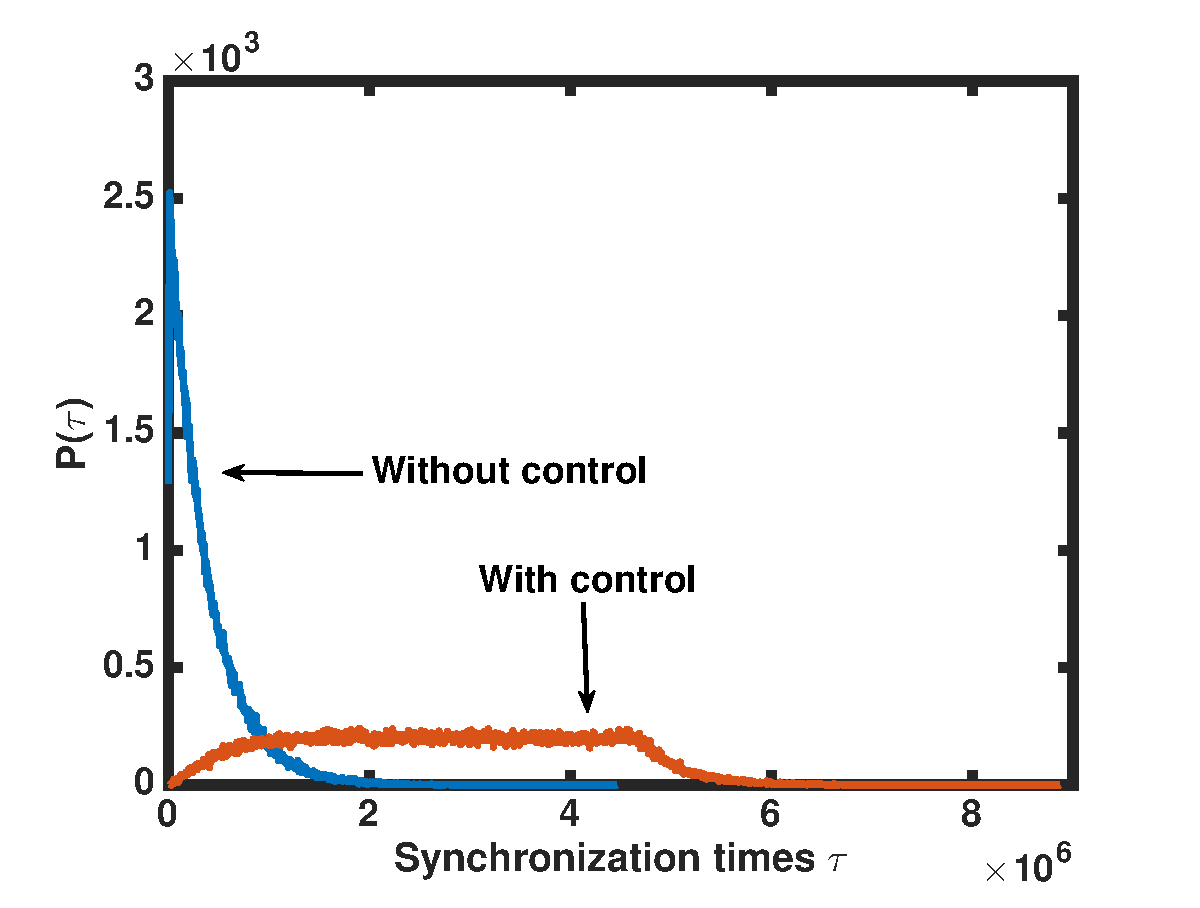
\includegraphics[scale=0.45]{Sync_time_dist.eps}
	\caption{\label{fig:Sync_time_dist}\footnotesize Distribution of 
		synchronization times without n-step control (the blue curve) and with 
		n-step 
		control (the red curve). The control delays synchronization times. }
\end{figure}

\begin{figure}[b]
    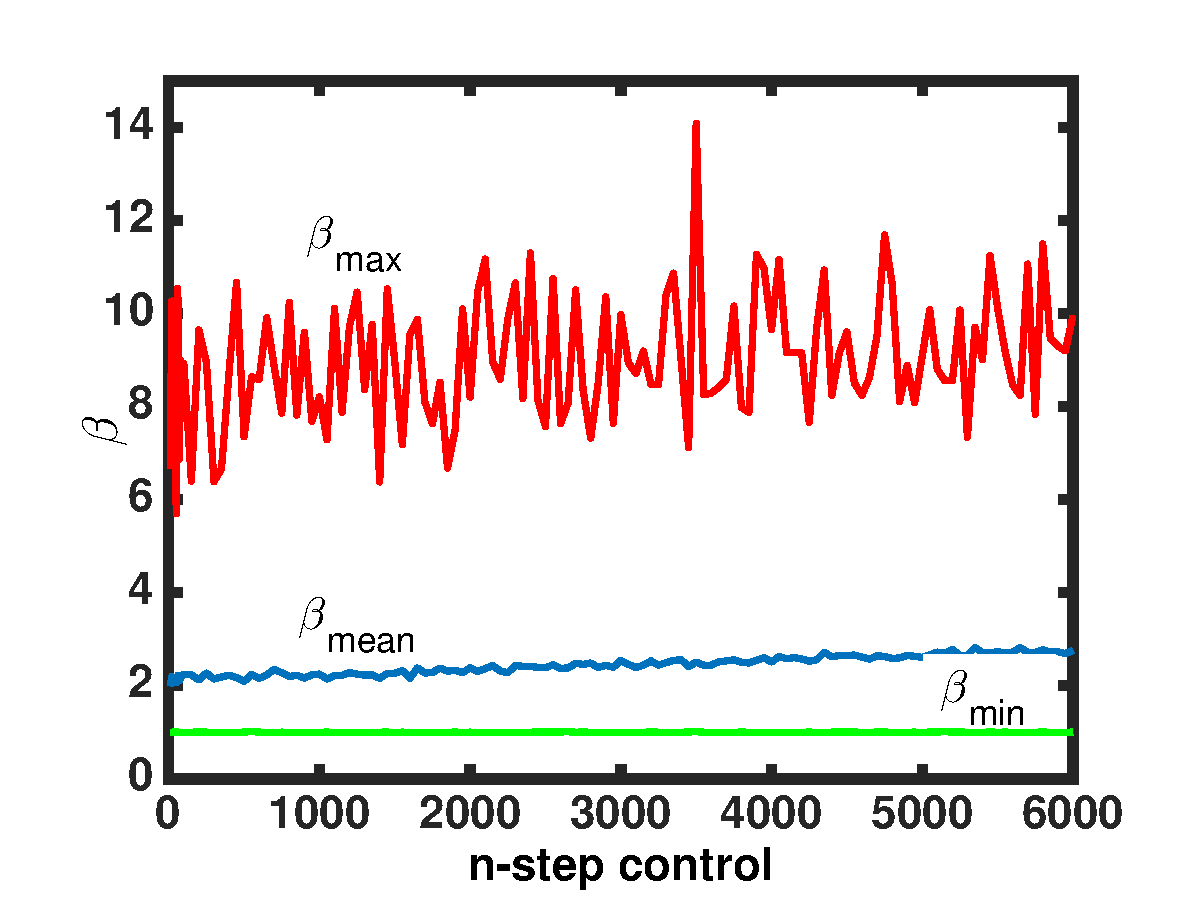
\includegraphics[scale=0.45]{Strength_con.eps}
    \caption{\label{fig:Strength_con}\footnotesize Variation of $\beta$ 
        (maximum, minimum and average) which measures the strength of 
        successful 
        delays i.e. $\beta = \ln(\frac{\tau_d}{\tau_0}$). $\beta_{max}$ 
        indicates the maximum delay time obtained at a give n-step control 
        while $\beta_{mean}$ stands for the mean value around 2. This means 
        that on an average, synchronization times re delayed by 100 times. The 
        minimum value of $\beta$ remains 1 for the cases when no delay was 
        obtained. }
\end{figure}

Fig.~\ref{fig:Control_success} shows the percentage of successful delays 
\textbf{(S)} (on the y-axis) for a given $n-$step control (on the x-axis) up 
to $n = 5500$ after which the successful cases are always $100\%$.  We achieve 
about $50\%$ successful cases for $n = 10$, which rises rapidly to $99\%$ for 
$n = 2950$. It is to be noted that the average synchronization time without 
any control, $\tau_{avg} \sim 10^5$. Therefore, the n-steps required to obtain 
all successful delays is just about $3\%$ of $\tau_{avg}$. We also plot the 
distribution of synchronization times for successful cases and compare it 
against that of corresponding times without control in 
Fig~\ref{fig:Sync_time_dist}. The long-tailed 
distribution of times without delay crosses over to a distribution which shows 
large flat region before a tail. The flat region indicate large number of 
successfully applied control with typical delay times of the order of $10^6$. 
For completeness, we show the decay in the number of undesired cases 
\textbf{U} in Fig~\ref{fig:Control_success}.  The cases \textbf{F} and 
\textbf{N} which are largely present for $n<10$, are extremely small in number 
and are neglected.


The degree of controlled synchronization $\beta$ may be defined as the ratio 
of synchronization times without numerical control, $\tau_c$ to 
synchronization times $\tau_0$ without control, i.e. $\beta =  
\ln(\frac{\tau_d}{\tau_0}$).  Therefore, for successfully delayed 
synchronization $\beta>0$ indicating $\tau_c > \tau$.The plot in 
Fig.~\ref{fig:Strength_con} shows the variation of $\beta$ i.e. $\beta_{min}$, 
$\beta_{mean}$, and $\beta_{max}$  indicating minimum, mean and maximum 
$\beta$ for considered $n-$step controls. Clearly, we are able to attain 
$\beta_{max}$ values to be in the range $5$ to $14$ while mean values remain 
$\sim2$. Therefore, we are successful in achieving 
significantly large delays in synchronization times. 


There are a couple of limitations of the proposed control procedure. The deflection to the trajectory visiting the sticky domain should not insert it inside the regular island. The regular trajectories of the drive and response map are known to synchronize significantly faster and would result in the undesirable possibility \textbf{(U)}. Therefore, an estimate of the size of regular islands, in addition to their locations must be known. These may be determined efficiently, as we have shown, using the edge-detection algorithm. The deflection area  may then be chosen suitably.  Another limitation is that the procedure is unable to impose a pre-determined delay to synchronization times. The random deflections simply keep the trajectories temporarily away from the synchronization traps in the sticky domain and synchronization may eventually occur after the removal of the control. 


\section{Advanced Synchronization Times}
\label{sec:advanced}
Based on the now explore the possibility to decrease synchronization times 
i.e. to expedite the process of synchronization. Once again, we will make use 
of the fact that synchronization traps typically exist in the sticky 
neighborhoods of the regular islands.  The procedure is based on the parameter 
perturbation technique to generate coherent structures in the phase space of 
an area-preserving map. However, the technique may also be used to push the 
chaotic bulk on the coherent structure (regular region) already present in the 
phase space and therefore, to make it disappear completely.  We describe the 
procedure briefly. 

\begin{figure*}[t]
    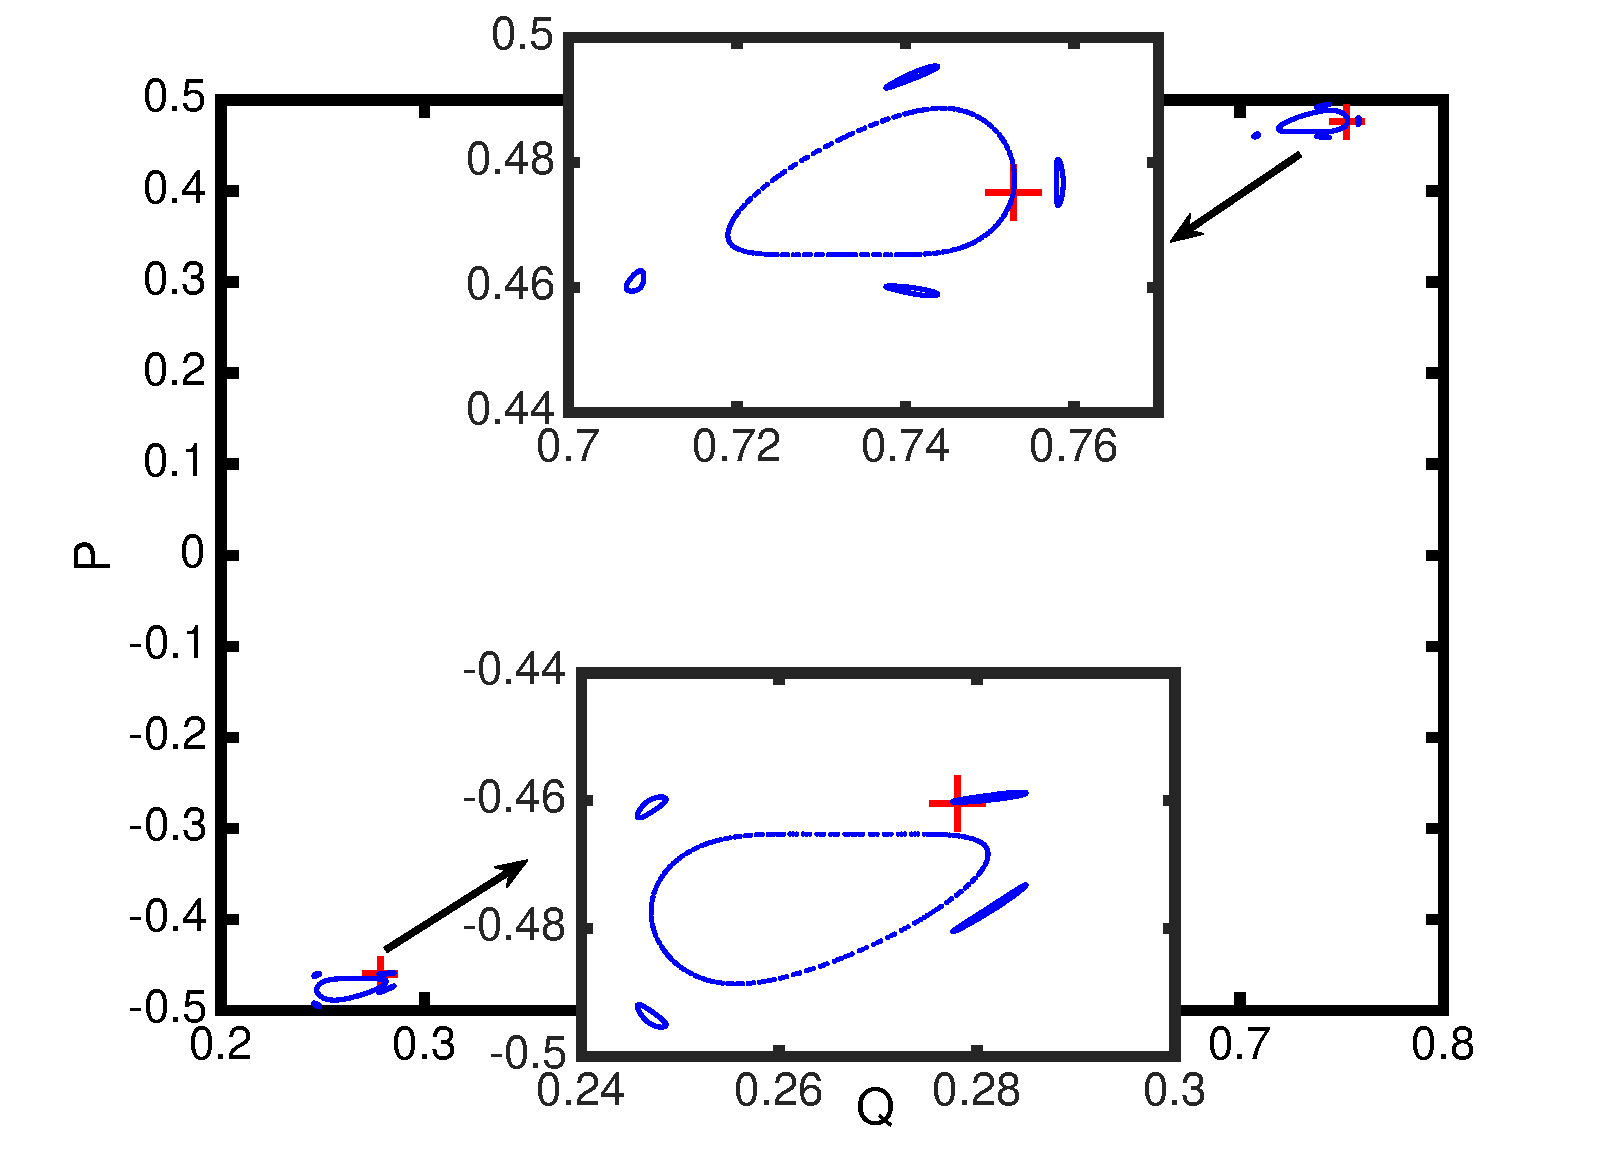
\includegraphics[scale=0.5]{Fast_sync_location.eps}
    \caption{\label{fig:location}\footnotesize The phase space of the drive 
        map at K = 6 for a couple of initial conditions where parameter 
        perturbation is applied. Synchronization occurs at the location 
        indicate 
        by the red `plus' signs.}
\end{figure*}
In a given area-preserving map, for instance, the  standard map, a  
perturbation in the nonlinearity parameter $K$ in the neighborhood of a 
suitable chosen periodic point leads to generation of large coherent 
structure.   We take the same form the standard map with a modulo operation 
such that $-0.5 \leq P_n \leq 0.5, 0\leq Q_n \leq 1$ . In this form, the 
standard map is known to have a hyperbolic fixed point at 
$(0,0)$,$(0,0.5)$. We perturb the parameter $K$ to $K-\epsilon$ if $|P - P_f| 
< \delta$, $|Q-Q_f| < \delta$. For $P$ and $Q$ outside this $\delta$-strip, 
$K$ does not change.  It may be noted that the perturbed standard map remains 
to be area-preserving. The Jacobian $J$ is now given by: 

\begin{minipage}[t]{0.45\textwidth}
	%\raggedleft
	\centering
	\[ J = \left( \begin{array}{cc}
	1 & 1 + (K-\epsilon)\cos(2\pi Q_n)   \\
	1 & (K-\epsilon)\cos(2\pi Q_n) \end{array} \right)\] 
\end{minipage}

\vspace{0.2cm}
	where, $ \epsilon \neq 0$ if $|P_f - P_n| < \delta$, $|Q_f - Q_n| < 
	\delta$\\ $\epsilon = 0$, otherwise.\\

The determinant of this matrix $J$ remains 1. The phase space thus obtained 
for for $K = 6$ , $\delta = 0.4$ and $\epsilon = 2$ for the fixed point 
$(P_f,Q_f)=(0.0,0.0)$ is shown in Fig.~\ref{fig:location}.   We have also 
performed computation for the other fixed point and with other modulo 
operations as well and results do not differ significantly. Our choice here of 
modulo operation and the fixed point $(P_f,Q_f)$ has some advantage over the 
others in terms of actual numerical values of synchronization times and the 
display of locations of the points where synchronization occurs. 

For the computations, we take 5 000 initial conditions chosen randomly from 
the chaotic region of the unperturbed standard map i.e. $P_0 \in \{-0.4,0.4\}$ 
and $Q_0 \in \{0.3,0.7\}$. The total number of iterations used for each 
initial condition to check for synchronization is $10^7$ and threshold of 
synchronization is $10^{-5}$ as previously.  The procedure has 
been applied to both drive and 
response map in accordance with our coupling  scheme described above. We 
choose a patch around $(P_f,Q_f)$  of length $\delta= 0.4$ which corresponds 
to about $16\%$ of the phase space area. We successfully obtain advance 
synchronization in more than $99.5\%$ of the cases among which a  couple of 
instances  has been shown in Fig.~\ref{fig:location} -- synchronization occurs 
in the neighborhood of one of the regular islands and one of their satellite 
islands.  The sign `+' in red indicate the point of synchronization. For 
details for the synchronization process, see ~\cite{Mahata2016,Das2017}.
\begin{figure}[h]
    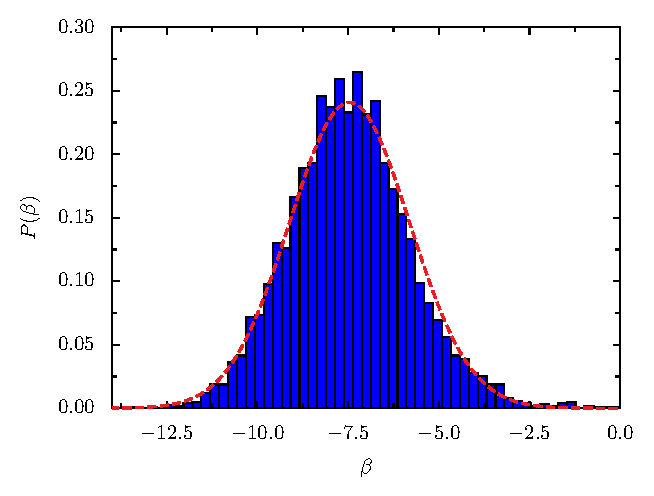
\includegraphics[scale=0.8]{sync_time_beta.eps}
    \caption{\label{fig:beta_dist}\footnotesize Distribution of degree of 
        controlled synchronization, $P(\beta)$, mean is -7.46 and standard 
        deviation is 1.67.}
\end{figure}
We again define the degree of controlled synchronization as $\beta = \ln 
(\frac{\tau_c}{\tau}$). For advanced synchronization, $\beta < 0$ indicating 
that synchronization times upon parameter perturbation is smaller than in 
normal course i.e. $\tau_c < \tau$. The normalized probability distribution of 
$\beta$ in shown in Fig.~\ref{fig:beta_dist}, which may be fit with a Gaussian 
of the following form:
\begin{equation}
f(\beta) =  a\exp\Big(-\frac{(\beta-\mu)^2}{2\sigma^2}\Big)
\end{equation}

We estimate the mean value $\mu \sim -7.46$ and standard deviation $\sigma 
\sim1.67$ which corresponds to the fact that, on an average, advanced 
synchronization times thus obtained are about $10^3$ times smaller than the 
normal synchronization times with $95.5\%$ values are between $10$ to $10^5$ 
times smaller.  Therefore, the synchronization times we obtained upon 
parameter perturbation is significantly smaller than the normal 
synchronization times.

The parameter perturbation technique is an efficient way to decrease synchronization times with high accuracy.  The value of the perturbation imposed should be chosen suitably as a very small may not have any influence on the synchronization process. The procedure also depends on the size and location of the patch wherein the control is applied. We are yet to see if the other technique of generating coherent structures also influence synchronization in these unidirectionally coupled systems. 


\section{Conclusions}
\label{sec:conclusions}
To summarize, we have developed numerical procedures to control 
synchronization in two identical standard map coupled under the drive-response 
configuration. The procedure is based on the fact that synchronization in the 
system typically occurs in the sticky neighborhoods of the regular islands in 
the phase space. We have shown that a delay in synchronization can be obtained 
by kicking the trajectories slightly away from the domain temporarily. The 
efficiency of the procedure depends upon the number of steps employed in 
control. By applying the procedure to the system on merely $1\%$ of the phase 
space area (at $K = 6$), we have successfully increased synchronization times. 
The maximum number of control steps that are used is $0.01\%$ of the total of 
number of iterations used throughout the computation.  Furthermore, the 
procedure gives variety of delays. The limitations of this procedure are, one, 
the deflection may insert the drive trajectory in the regular islands which 
would lead to undesirable faster synchronization and two, a predetermined 
synchronization time in not obtainable. Furthermore, we have demonstrated a 
simple way to fasten synchronization by the parameter perturbation technique 
which rapidly drives the chaotic trajectories in the sticky neighborhood of 
regular islands. The distribution of degree of controlled synchronization 
times indicates the efficiency of the procedure. In both the numerical 
procedures, we have ignored the complex hierarchical structures which lead to 
sticky behavior of the chaotic orbits in the phase space. A possible future 
direction is to investigate the role of stickiness in measure synchronization 
in coupled Hamiltonian systems.

\begin{acknowledgments}
I would like to thank Neelima Gupte and Arnd B\"acker for their suggestions to improve the manuscript. 
\end{acknowledgments}




\appendix
%%%%%%%%%%%%%%%%%%%%%%%%%%%%%%%%%%%%%%%%%%%%%%%%%%%%%%%%%%%%%%%%%%%%%%%%%%%%%
%\section{Some stuff for the appendix}
%%%%%%%%%%%%%%%%%%%%%%%%%%%%%%%%%%%%%%%%%%%%%%%%%%%%%%%%%%%%%%%%%%%%%%%%%%%%%


%%%%%%%%%%%%%%%%%%%%%%%%%%%%%%%%%%%%%%%%%%%%%%%%%%%%%%%%%%%%%%%%%%%%%%%%%%%%%
%\bibliographystyle{cpg_unsrt_title}
%\bibliographystyle{cpg_unsrt_key_title}
%\bibliographystyle{cpg_unsrt_title2}
%\bibliographystyle{cpg_unsrt_key_title2}
%\bibliographystyle{unsrt}
\bibliographystyle{cpg_unsrt_title_for_phys_rev}
%\bibliographystyle{cpg_unsrt_key_title2} % to have labels + links


% See ~/Devel/Repositories/Bibtex/notes.txt
% if you need more
\bibliography{Syncref}




\end{document}
